\section{Nicht gleichförmig reduzierte zeiterweiterte Netzwerke}\label{sec:nonunif_cond}
Die gleichmäßige Unterteilung der Zeit durch $\timeDom = \{0,1, \ldots, T-1\}$ kann bei
anderen Problemen zu schlechten Ergebnissen führen. Wir wollen dazu kurz das Problem
des „Earliest-Arrival-Flows“ und dazu ein kritisches Beispiel betrachten.

\begin{problem}[Earliest-Arrival-Flow]
\label{prob:qtp_single}
    Sei ein Netzwerk $(\graph, \tau)$ mit $K=\{1\}$ und einer Senke $t$, sowie
    $T > 0$ gegeben.

    Gesucht ist ein Fluss $f^*$, der zu jedem Zeitpunkt $t \in \ropen{0,T}$
    maximal ist.
\end{problem}

Wir haben gesehen, dass ein statischer Fluss in $\tExp{T}$ als dynamischer Fluss
interpretiert werden kann. Dies ergibt einen Fluss, der stückweise konstant ist.
Danach wurde ein solcher Fluss über ein Zeitintervall verteilt. Dies kann
aber zu Problemen führen:

\begin{example}
    Wir betrachten das Netzwerk aus \figRef{ex_non_uniform}.
    \begin{figure}[H]
    \centering
    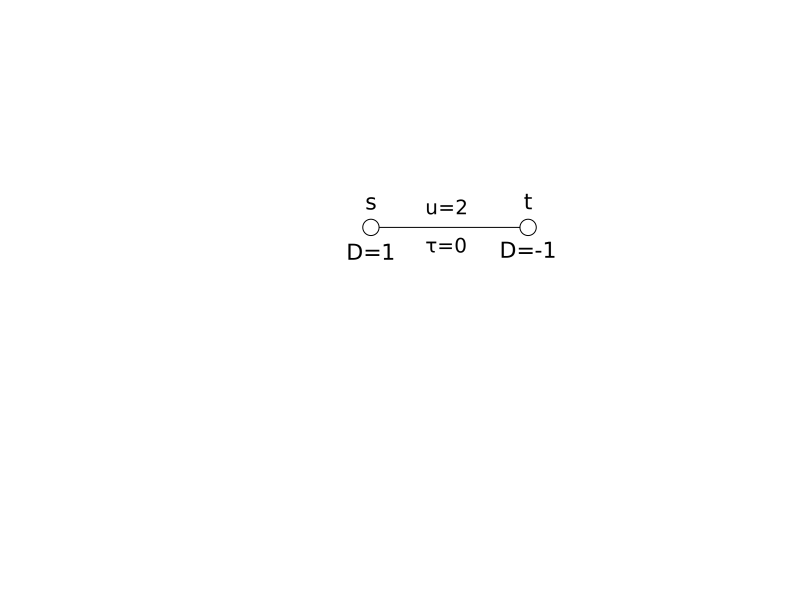
\includegraphics[width=0.4\textwidth]{ex_non_uniform}
    \caption{Beispiel für ein Netzwerk, in dem die Zeit nicht mit ganzen
                Zahlen unterteilt werden kann}
    \label{fig:ex_non_uniform}
    \end{figure}
    Um den Bedarf zu erfüllen und möglichst früh den höchsten Fluss
    zu haben, wäre
    \[
        f(t) = \begin{cases}
            2, t \in \ropen{0,\frac{1}{2}} \vspace{3pt} \\
            0, t \in \ropen{\frac{1}{2}, 1}
        \end{cases}
    \]
    eine Lösung für das Earliest-Arrival-Problem.

    Wählen wir als Zeitunterteilung Intervalle der Länge $1$, muss dieser Fluss
    über einen Zeitraum von $1$ gemittelt werden. Also ergibt sich der Fluss
    $\widetilde{f}(t) = 1$. Dieser weicht aber um den Faktor $2$ von der
    besten Lösung ab.
\end{example}

Man kann dieses Problem umgehen, indem man den Zeitverlauf anders unterteilt. In dem
Beispiel würde die Unterteilung in Intervalle der Größe $\frac{1}{2}$
genügen ($\timeDom = \{0, \frac{1}{2}, 1\}$). Wir wollen uns für diesen Fall nur
die entsprechende Definition des zeitertweiterten Netzwerks ansehen.

\begin{definition}[Zeiterweitertes Netzwerk mit beliebigen Zeitintervallen]
    Sei $(\graph, \tau)$ und $L = (\theta_q)_{q \in R}$, wobei $R = \{0, \ldots, r\}$,
    sodass
    \[
        0 = \theta_0 < \theta_1 < \ldots < \theta_r < T.
    \]
    Setze $\theta_{r+1} = T$.
    Dann ist das \term{L-zeiterweiterte Netzwerk} $\tExp{L} = (V^L, \A^L)$
    gegeben durch
    \begin{itemize}
        \item $V^L = V \times R$ (schreibe $v_q = (v, q)$ und
            $V_q = \{v_q \in V^L\}$)
        \item $\A^L = \setDef{e_q = (v_q, u_{m(e, q)})}
                        {e = (v, u) \in \A, q \in R, \theta_q + \tau(e) \leq \theta_r}
                    \cup H$, \\
            \text{ wobei } $H = \setDef{(v_q, v_{q+1})}
                                    {v \in S_i \text{ und } q, q+1 \in R}$
    \end{itemize}

    Dabei ist $\func{m}{\A \times R}{R}$ definiert durch
    \[
        m(e, q) := \min \setDef{q' \in R}{\theta_q + \tau(e) \leq \theta_{q'}}.
    \]
    $m$ bestimmt also das Intervall, zwischen welchen die Kante $e$ transportiert.
    Der Rest ist analog wie bei den ursprünglichen zeiterweiterten Netzwerken
    definiert.
\end{definition}

\begin{remark}
    Offensichtlich ergibt sich mit einer Unterteilung $L = (0, 1, \ldots, T-1)$
    wieder $\tExp{T} = \tExp{L}$. Also sind L-zeiterweiterte Netzwerke
    eine Verallgemeinerung.
\end{remark}

Mit dieser Konstruktion kann auch für Earliest-Arrival-Flows eine \\
$(1+\eps)$-Approximation bestimmt werden. Siehe dazu \cite[5.2]{fleischerSiam}.
% TODO: wie werden diese benutzt?
